% Configuração do tipo de documento
\documentclass{article}

% Configuração do idioma
\usepackage[utf8]{inputenc}
\usepackage{lipsum}
\usepackage{graphics}
\usepackage{tcolorbox}
\usepackage{helvet}
\usepackage{setspace}
\usepackage{hyperref}
\usepackage{media9}

% Ajustar espaçamentos ao redor do texto
\usepackage{geometry}
\geometry{
    a4paper,
    left=2.5cm,
    right=2.5cm,
    top=3cm,
    bottom=3cm
}

% Configuração do cabeçalho e rodapé
\usepackage{fancyhdr}
\pagestyle{fancy}
\fancyhf{}
\lhead{
\includegraphics[width=0.5cm]{./images/appService.png} \space\space Canto esquerdo}
\chead{No centro \space\space 
\includegraphics[width=0.5cm]{./images/appService.png} \space\space No centro}
\rhead{Canto direito \space\space 
\includegraphics[width=0.5cm]{./images/appService.png}}
\lfoot{
\includegraphics[width=0.5cm]{./images/appService.png} \space\space Rodapé esquerdo}
\cfoot{Rodapé central \space\space 
\includegraphics[width=0.5cm]{./images/appService.png} \space\space Rodapé central}
\rfoot{Página \thepage \space\space 
\includegraphics[width=0.5cm]{./images/appService.png}}

% Configuração da fonte e espaçamento - Abnt
\renewcommand{\familydefault}{\sfdefault}
\onehalfspacing

% Configuração do título
\title{\bfseries\fontsize{16}{16}\selectfont Título do Artigo}
\author{}
\date{}
    
% Início do documento
\begin{document}

% Adição de imagem
\begin{figure}[h]
    \centering
    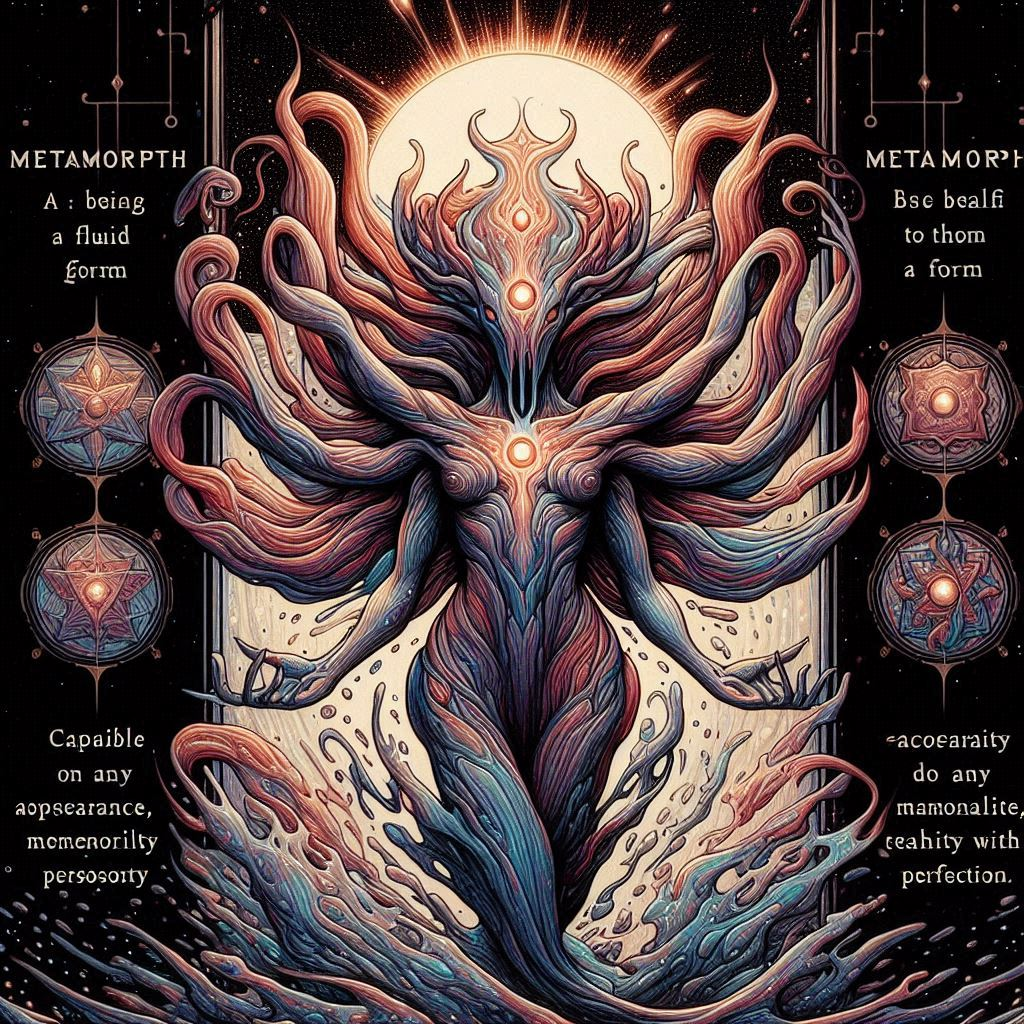
\includegraphics[width=0.5\textwidth]{./images/Metamorph_All.jpeg}
    \maketitle
\end{figure}
\newpage

% Inclusão do sumário
\renewcommand{\contentsname}{Sumário}
\tableofcontents
\newpage

% Inclusão de seção
\section{Introdução}
\lipsum[1]

% Inclusão de tabela justificada
\begin{table}[h]
    \centering
    \begin{tabular}{|p{5cm}|p{5cm}|p{5cm}|}
        \hline
        Coluna 1 & Coluna 2 & Coluna 3 \\
        \hline
        1 & 2 & 3 \\
        \hline
        4 & 5 & 6 \\
        \hline
        7 & 8 & 9 \\
        \hline
    \end{tabular}
    \caption{Exemplo de tabela justificada}
\end{table}

% Exemplo de conteúdo JSON
\begin{tcolorbox}
\begin{verbatim}
{
    "key1": "value1",
    "key2": "value2",
    "key3": "value3"
}
\end{verbatim}
\end{tcolorbox}

% Inclusão de seção
\section{Desenvolvimento}
\lipsum[2]

% Inclusão de tópico
\subsection{Sub-tópico 1}
\lipsum[1]

% Inclusão de sub-tópico
\subsubsection{Subsub-tópico 1}
\lipsum[1]

% Inclusão de Link com aparência de link
\href{https://www.google.com}{\textbf{\textcolor{blue}{\underline{Google}}}}

% Inclusão de sub-tópico
\subsubsection{Subsub-tópico 2}
\lipsum[1]

% Inclusão de tópico
\subsection{Sub-tópico 2}
\lipsum[2]

% Inclusão de tópico
\subsection{Sub-tópico 3}
\lipsum[3]

% Inclusão de lista não enumerada
\begin{itemize}
    \item Item 1
    \begin{itemize}
        \item Subitem 1
        \item Subitem 2
        \begin{itemize}
            \item Subsubitem 1
            \item Subsubitem 2
        \end{itemize}
    \end{itemize}
    \item Item 2
    \item Item 3
\end{itemize}

% Inclusão de seção
\section{Conclusão}
\lipsum[3]

% Inclusão de lista enumerada
\begin{enumerate}
    \item Item 1
    \begin{enumerate}
        \item Subitem 1
        \item Subitem 2
        \begin{enumerate}
            \item Subsubitem 1
            \item Subsubitem 2
        \end{enumerate}
    \end{enumerate}
    \item Item 2
    \item Item 3
\end{enumerate}

% Fim do documento
\end{document}